% !TEX encoding = UTF-8 Unicode
\documentclass[
11pt,
master, % тип документа
subf, % подключить и настроить пакет subfig для вложенной нумерации рисунков
href, % подключить и настроить пакет hyperref
colorlinks=true, % цветные гиперссылки
times, % шрифт Times как основной
%fixint=false % отключить прямые знаки интегралов
]{disser}
\usepackage[left=25mm, top=20mm, right=10mm, bottom=20mm]{geometry}
\usepackage[T2A]{fontenc}
\usepackage[utf8]{inputenc}
\usepackage[english,russian]{babel}
\usepackage{amsmath,amssymb,cmap} % cmap для кодировки шрифтов в pdf
\usepackage{pdfpages} % вставляем pdf файлы
\usepackage{indentfirst} % отделять первую строку раздела абзацным отступом
\usepackage{titletoc} % убираем отступ перед "Оглавление"
\usepackage{graphicx}
\usepackage{setspace}
\usepackage{verbatim} % для оформления кода
\usepackage{pdfsync} % установка соответствия документ - код
\graphicspath{{./Img/}}

\setlength\parindent{5ex} % абзацный отступ равный пяти строчным буквам основного шрифта
\pagestyle{plain} % включаем нумерацию
\setcounter{tocdepth}{2} % включать подсекции в оглавление
\linespread{1.3} % полуторный интервал


% Номера страниц снизу и по центру
\pagestyle{footcenter}
\chapterpagestyle{footcenter}

\begin{document}
	
\pagestyle{empty}
\begin{center}
	
	\noindent  Федеральное государственное бюджетное образовательное учреждение\\
	высшего профессионального образования\\
	
	Московский государственный технический университет им. Н.Э. Баумана \\
	Факультет <<Фундаментальные науки>>\bigskip\\
	
	\vfill
	
	Лабораторная работа №6\\
	по курсу «Вычислительная физика»\\
	Тема: «Метод Монте Карло»\\
	\textbf{Вариант 6}\\
	
	
	\vfill
	\vfill
	\begin{flushright}
		\begin{tabular}{ll}
			Выполнили: & студенты группы ФН4-72Б     \\
			& Мистрюкова Л.А., Хижик А.И.  \\
			Проверил:  & доцент, к.физ.-мат.н.       \\
			& Хасаншин Р.Х.
		\end{tabular}
	\end{flushright}
	\vfill
	\begin{center}
		Москва, $2019$
	\end{center}
	
\end{center}
\pagebreak
	
	
\pagestyle{plain}
\tableofcontents

\section{Теоретическая часть}
\subsection{Введение}
С развитием вычислительной техники возрастает интерес к численным методам решения прикладных задач, в частности к статистическому моделированию (или методу Монте-Карло (ММК)). Исторически интенсивное развитие теории и приложений ММК было связано с решением актуальных задач теории переноса излучения в 50-х годах XX в. За последние полвека сфера применимости методов численного статистического моделирования значительно расширилась. Разработана теория вероятностных представлений решений задач математической физики, на основе которой построены соответствующие численные стохастические оценки. Эффективные алгоритмы разработаны также в статистической физике (метод Метрополиса, схема Изинга), физической и химической кинетике (многочастичные задачи, решение уравнений Больцмана и Смолуховского, моделирование реакций и фазовых переходов), теории турбулентности и др.

Под численным статистическим моделированием обычно понимают реализацию с помощью компьютера вероятностной модели некоторого объекта с целью оценивания изучаемых интегральных характеристик на основе закона больших чисел.

В самом общем виде схема ММК выглядит следующим образом. Пусть требуется вычислить некоторую величину $I$. Предполагается, что можно построить случайную величину $\zeta$ с математическим ожиданием $M[\zeta]$, равным $I$, и с конечной дисперсией $D[\zeta]$, причём выборочные значения $\zeta_i$ случайной величины $\zeta$ достаточно просто реализуются на компьютере. Построив большое количество $N$ выборочных значений $\zeta_1,\ldots,\zeta_N$ на основе закона больших чисел получаем приближение искомой величины
$$I = M[\zeta] \approx \overline{\zeta}_N = \frac{\zeta_1 + \ldots + \zeta_N}{N}.$$

\textbf{Основные особенности ММК}:\\
1. Простота вычислительного алгоритма\\
Как правило составляется программа для реализации одного испытания. Эта процедура повторяется $N$ раз и результаты испытаний усредняются.\\
2. Погрешность метода пропорциональная $\sqrt{\frac{D}{N}}$, где $D$ -- дисперсия, $N$ -- статистика (число испытаний). Нетрудно заметить, что скорость сходимости достаточно мала.

\subsection{Стандартный ММК}
Пусть требуется приближённо вычислить $l$-кратный интеграл
\begin{equation}\label{eq1}
  I = \int_{R^l} g(x)dx,
\end{equation}
где $dx = dx_1 \ldots dx_l$. Зачастую (\ref{eq1}) удобнее записывать в виде $I =\int_{X} g(x) dx$, где $X$ -- замыкание множества тех $x\in R^l$, для которых $g(x)\neq 0$.

Выберем плотность распределения $p_{\xi}(x)$ случайного вектора $\xi =(\xi_1,\ldots,\xi_l)$ в $R^l$, такую, что
$$p_{\xi}(x)\geq 0,\;\; \int_{R^l} p_{\xi}(x)dx = 1.$$
Перепишем интеграл (\ref{eq1}) в виде математического ожидания
\begin{equation}\label{eq2}
  I = \int_{R^l}g(x) dx = \int_{R^l}\eta(x)p_{\xi}(x)dx = M[\zeta],
\end{equation}
где $\eta(x) = \frac{g(x)}{p_{\xi}(x)}$, $\zeta = \eta(\xi).$

Рассмотрим набор $\{\xi_i\}$ из $N$ одинаково распределённых случайных векторов с плотностью распределения $p_{\xi}(x)$. Предположим, что они независимы, тогда случайные величины $\{\zeta_i\}$, $\zeta_i = \eta(\xi_i)$, $i=\overline{1,N}$ будут также независимыми одинаково распределёнными с математическим ожиданием $I$ и дисперсией $D$. Для $\zeta_{\Sigma} = \sum_{i=1}^{N} \zeta_i$ математическое ожидание $M[\zeta_{\Sigma}] = NI$ и дисперсия $D[\zeta_{\Sigma}] = ND$

Согласно центральной предельной теореме, для бесконечной последовательности независимых одинаково распределённых случайных величин $\{\zeta_i\}$, имеющих конечное математическое ожидание $M$ и дисперсию $D = \sigma^2$ имеет место предел
$$\frac{\overline{\zeta_\Sigma}-M}{\sigma}\sqrt{N} \underset{N\rightarrow \infty}\rightarrow\mathcal{N}(0,1),$$
где $\overline{\zeta_\Sigma} = \frac{\zeta_\Sigma}{N}$, $\mathcal{N}(0,1)$ -- нормальное распределение с нулевым математическим ожиданием и стандартным отклонением, равным единице. Данное утверждение позволяет использовать правило 3-сигм:
$$P\left\{NI-3\sqrt{ND} < \zeta_\Sigma < NI + 3\sqrt{ND}\right\} \approx 0.997,$$
\begin{equation}\label{eq3}
  P\left\{\left|\frac{1}{N}\sum_{i=1}^{N}\frac{g(\xi_i)}{p_{\xi}(\xi_i)}-I\right| < 3\sqrt{\frac{D}{N}}\right\} \approx 0.997.
\end{equation}
\begin{equation}\label{eq4}
  I \approx \frac{1}{N}\sum_{i=1}^{N}\frac{g(\xi_i)}{p_{\xi}(\xi_i)}.
\end{equation}

Формулы (\ref{eq3}-\ref{eq4}) предлагают способ вычисления интеграла и вероятностную оценку ошибки.
\begin{equation}\label{eq5}
  \sigma^2 = D[\zeta] = M[\eta^2(\xi)] - (M[\eta(\xi)])^2 = \int_{R^l} \eta^2(x) p_{\xi}(x)dx - I^2 = \int_{R^l}\frac{g^2(x)}{p_{\xi}(x)}dx - I^2.
\end{equation}

Из соотношения (\ref{eq3}) следует, что скорость сходимости ММК определяется величиной $N^{-1/2}$, т. е. относительно невелика. При вычислении однократного интеграла $I$ с гладкой подынтегральной функцией $g(x)$ для $x \in [a, b]$ погрешность простейшей формулы прямоугольников, определяемая числом $N$ вычислений подынтегральной функции $g(x)$ из (\ref{eq1}), имеет порядок $N^{-2}$, а формула Симпсона имеет ещё более высокий порядок погрешности $N^{-3}$. Упомянутые формулы являются частными случаями так называемых квадратурных формул Ньютона—Котеса, построение которых основано на интегрировании полиномиальных интерполяций подынтегральной функции $g(x)$. Хорошо известно, что при переходе к размерностям $l$ интеграла (\ref{eq1}), больших единицы, и при рассмотрении негладких подынтегральных функций $g(x)$, $x \in R^l$, построение интерполяций для $g(x)$ и соответствующих им кубатурных формул значительно усложняется и порядок $t$ погрешности $\delta_n \sim N^{-t}$ уменьшается с ростом $l$. Скорость сходимости $N^{-1/2}$ ММК не зависит от размерности $l$ (эта скорость сохраняется, в том числе и для интегралов бесконечно возрастающей кратности). Свойства функции $g(x)$ влияют лишь на величину $D\zeta$ из (\ref{eq5}).

Таким образом, при переходе к сложным многомерным задачам конкурентоспособность ММК возрастает. Принято считать, что для $1<l<3$ предпочтительнее использовать кубатурные формулы, для $l>10$ не имеет конкурентов простейший ММК или его модификации. Для размерностей $3<l<10$ имеет смысл рассматривать смешанные дискретно-стохастические методы численного интегрирования.

\subsection{Трудоемкость ММК}
Важным преимуществом метода Монте-Карло является простота учёта вычислительных затрат, позволяющая проводить оптимизацию за счёт специального выбора плотности $p_{\xi}(x)$. Действительно, затраты на вычисление величины $\zeta$ равны $s=nt$, где $t$ — среднее время для получения одного выборочного значения $\zeta_i$ случайной величины $\zeta$ (затратами на суммирование и деление на $N$ в формуле (\ref{eq4}) можно пренебречь). Полагая, что величина $\frac{3\sigma}{\sqrt{N}}$ из (\ref{eq3}) определяет погрешность $\delta_N = \delta = const$:
$$N = A\sigma^2;\;\; A = \frac{9}{\delta^2}.$$
Следовательно, число испытаний $N$ пропорционально дисперсии $\sigma^2 = D[\zeta]$, поэтому можно заменить величину $s$ на
\begin{equation}\label{eq6}
  S = t \times D[\zeta].
\end{equation}

Величина (\ref{eq6}), называемая трудоемкостью метода Монте-Карло, является критерием качества алгоритма. Тот выбор плотности $p_{\xi}(x)$ считается лучше, для которого величина $S$ меньше.

Неизвестная величина $\sigma = \sqrt{D[\zeta]}$, из (\ref{eq5}) допускает эффективное оценивание с помощью реализуемых выборочных значений $\zeta_1,\ldots,\zeta_N$. Простейшее приближение несложно получить из соотношения (\ref{eq2}) для $\eta(u) = u^2$:
\begin{equation}\label{eq7}
  D[\zeta] = M[\zeta^2] - (M[\zeta])^2 \approx D_N^{(1)} = \frac{1}{N}\sum_{i=1}^{N} \zeta^2_i - \left(\frac{1}{N} \sum_{i=1}^{N} \zeta_i\right)^2.
\end{equation}

Если в (\ref{eq7}) трактовать $\zeta_1,\ldots,\zeta_N$ как независимые и одинаково распределённые (так же как случайная величина $\zeta$) случайные величины, то несложно показать, что
\begin{equation}\label{eq8}
  M\left[D_N^{(1)}\right] = \left(1-\frac{1}{N}\right)D[\zeta].
\end{equation}
Действительно, $M\left[D_N^{(1)}\right] = M\left[\zeta^2\right] - M\left[\overline{\zeta}^2_N\right] = D[\zeta] - D\left[\overline{\zeta}_N\right]$, так как $M[\overline{\zeta}_N] = M[\zeta]$. Учитывая, что $D\left[\overline{\zeta}_N\right] = D\left[\frac{\zeta}{N}\right]$, получаем (\ref{eq8}). Несмещённую оценку дисперсии можно получить, разделив $D_N^{(1)}$ на $(1-1/n)$:
\begin{equation}\label{eq9}
  D_N^{(2)} = \frac{1}{N-1} \sum_{i=1}^{N}\zeta_i^2 - \frac{1}{N(N-1)}\left(\sum_{i=1}^{N}\zeta_i\right)^2.
\end{equation}

Замена в соотношении (\ref{eq3}) величины $\sigma$ на $\sqrt{D_N}$ изменяет «доверительную границу» $\frac{3\sigma}{\sqrt{N}}$ на величину порядка $O(1/N)$, если $M[\zeta^4]<+\infty$.

\subsection{Простейшие методы вычисления определённых интегралов}
\subsubsection{Вычисление среднего значения}
Рассмотрим случайную величину $\xi$ равномерно распределённую на $(a,b)$ с функцией распределения $p_{\xi}(x)$:
$$p_{\xi}(x) = \left\{
                 \begin{array}{ll}
                   \frac{1}{b-a}, & \hbox{$x\in (a,b)$;} \\
                   0, & \hbox{$x\overline{\in} (a,b)$.}
                 \end{array}
               \right.
$$

$$M[f(\xi)] = \int_{R} f(x)p_{\xi}(x)dx = \frac{1}{b-a} \int_{a}^{b} f(x)dx = \frac{I}{b-a} \Rightarrow I = (b-a)M[f(\xi)].$$

Таким образом, если взять достаточно большое $N$ значений случайной величины $\xi$: $\{\xi_i\}$, то $M[f(x)] \approx \frac{1}{N} \sum_{i=1}^{N} f(\xi_i)$
\begin{equation}\label{eq10}
  I \approx Q_1 = \frac{b-a}{N}\sum_{i=1}^{N}f(\xi_i).
\end{equation}
Выражение (\ref{eq10}) -- сумма Дарбу со случайными узловыми точками.

\subsubsection{Вычисление площади}
Пусть функция $f$ ограничена: $0\leq f\leq C$. $(\xi,\eta)$ -- случайные величины равномерно распределённые в прямоугольнике $ABCD$: $\{(x,y)\colon a<x<b\vee0<y<C\}$.

Плотность вероятности $p_{\xi\eta} = \left\{
                                       \begin{array}{ll}
                                         \frac{1}{C(b-a)}, & \hbox{$(\xi,\eta) \in ABCD$;} \\
                                         0, & \hbox{$(\xi,\eta)\overline{\in}ABCD$.}
                                       \end{array}
                                     \right.$\\
Возьмём $N$ случайных точек и равномерно распределим их на поверхности прямоугольник, $N'$ - количество точек род кривой $f(x)$. Тогда $I\approx C(b-a)\frac{N'}{N}$.

Для того, чтобы разыграть следующую случайную точку необходимо получить значения случайных величин $\xi$ и $\eta$:
$$\xi_i = a + (b-a)\gamma_i,$$
$$\eta_i = C\gamma_{i+1}.$$

Алгоритм подсчета точек под кривой: $\left\{
                                      \begin{array}{ll}
                                        f(\xi_i) < \eta_i \rightarrow N_i = N_i, \\
                                        f(\xi_i) > \eta_i \rightarrow N_I = N_i + 1.
                                      \end{array}
                                    \right.$
\begin{equation}\label{eq11}
  I \approx Q_2 = C(b-a)\frac{N'}{N}.
\end{equation}

\subsubsection{Сравнение точности методов}
Метод 1: $\nu_1 = (b-a)f(\xi)$, $D[\theta] = \frac{D[\nu_1]}{N}$
\begin{equation}\label{eq12}
  D[\nu_1] = \int_{a}^{b}(b-a)^2f^2(x)p_{\xi}(x)dx - I^2 = (b-a)\int_{a}^{b} f^2(x)dx - I^2.
\end{equation}

Метод 2: $\nu_2 = C(b-a)g(\xi,\eta)$

$$g(x,y) = \left\{
             \begin{array}{ll}
               1, & \hbox{$y<f(x)$,} \\
               0, & \hbox{$y>f(x)$.}
             \end{array}
           \right.$$
\begin{equation}\label{eq13}
  D[\nu_2] = \int_{a}^{b} \int_{0}^{f(x)} (C(b-a)g(x,y))^2p(x,y)dxdy - I^2 = C(b-a)\int_{a}^{b}f(x)dx - I^2.
\end{equation}

Очевидно, метод 1 точнее метода 2.

\subsection{Методы понижения дисперсии}
\subsubsection{Выделение главной части}
Допустим, что известна близкая к $g(x)$ функция $g_0(x)$, для которой легко вычисляется интеграл $I_0 = \int g_0(x)dx$ (аналитически или численно с малыми затратами и высокой точностью). Тогда для увеличения эффективности расчётов ММК можно использовать стандартный прием выделения главной части, который основан на соотношении
$$I = I_0 + \int_{R^l}[g(x)-g_0(x)]dx.$$
Для оценки второго слагаемого применим построенный ранее алгоритм, следовательно,\\
$I=M\left[\zeta^{(0)}\right]$, где $\zeta^{(0)} = I_0 + \eta(\xi) - \eta_0(\xi)$, $\eta_0(\xi) = \frac{g_0(\xi)}{p_{\xi}(\xi)}$, а случайный вектор $\xi$ распределен согласно плотности $p_{\xi}(x)$.

Дисперсия $D\left[\zeta^{(0)}\right] = D(\eta(\xi)-\eta_0(\xi))$ и может быть малой, если $g_0(x)$ хорошо аппроксимирует функцию $g(x)$.

Если рассматриваемая случайная величина $\xi$ равномерно распределена на $(a,b)$, интеграл принимает вид:
\begin{equation}\label{eq14}
  I\approx \theta_3 = \frac{b-a}{N}\sum_{i=1}^{N}[f(\xi_i)-g(\xi_i)] + I_0.
\end{equation}

\subsubsection{Использование существенной выборки}
Оптимальным выбором плотности вероятности приводящим к минимуму дисперсии в формуле (\ref{eq5}), является плотность вероятности следующего вида: $\frac{|g(x)|}{\int_{a}^{b}|g(x)|dx}$.

На практике следует придерживаться правила: $\frac{p(x)}{|g(x)|} \approx const$. Для того, чтобы выполнялось это условие, иногда приходится прибегать к сложным функциям, что нерационально, так как усложняет моделирование значений случайных величин, то есть процедуру розыгрыша.

\subsubsection{Симметризации подынтегральной функции}
Под этим названием объединяются методы, построенные на использовании информации об интегрируемой функции.

Предположим, что необходимо вычислить $\int_{0}^{1}f(x)dx$ и подынтегральная функция $f(x)$ монотонна. Очевидно, что интеграл от $f(1-x)$ совпадает с интегралом от $f(x)$. Положим $g(x) = \frac{1}{2}[f(x) + f(1-x)]$, $g(x)$ -- имеет меньшую дисперсию, чем $f(x)$. Тогда

\begin{equation}\label{eq15}
  I\approx \theta_4 = \frac{1}{2N}\sum_{i=1}^{N}[f(\xi_i)+f(1-\xi_i)]
\end{equation}
Данный метод эффективен, если $D[\theta_1] > 2D[\theta_2]$

\newpage
\section{Постановка задачи}
\begin{itemize}
  \item Вычислить интегралы $\displaystyle\int_{0}^{1}\exp(x)dx$ и $\displaystyle\int_{0}^{\pi/2} \sin(x)dx$  с помощью ММК, используя простейшие методы и способы понижения дисперсии. Оценить соответствующие значения дисперсией.
  \item Вычислить интеграл $\displaystyle \int_{0}^{\sqrt{3}} x\arctan(x) dx$ из лабораторной работы №5 с помощью ММК. Сравнить полученный результат с результатами вычислений по формулам прямоугольников, трапеций и Симпсона.
\end{itemize}

\newpage
\section{Программа}

{\footnotesize
\begin{verbatim}
#include <iostream>
using namespace std;
#include <random>
#include <cmath>

const double PI = 3.141592653589793238463;
double a1 = 0, b1 = 1, c1 = exp(1), c11 = exp(1) - 2.5, c111 = 0.5 * (exp(1)+1);
double Integral1 = exp(1) - 1;  // точное значение интеграла для f1
double a2 = 0, b2 = PI/2, c2 = 1, c22 = 1 - PI/2 + pow(PI,3) / 48, c222 = PI / 4;
double Integral2 = 1;  // точное значение интеграла для f2
double a3 = 0, b3 = sqrt(3), c3 = sqrt(3) * atan(sqrt(3)), c33 = 7.985, c333 = PI / (2 * sqrt(3));
double Integral3 = (4 * PI - 3 * sqrt(3)) * 1 / 6;  // точное значение интеграла для f3
int N = 10000;
double f1(double x); // интегрируемая функция
double fg1(double x); // функция для выделения главной части
double fs1(double x); // симметризованная функция
double f2(double x);
double fg2(double x);
double fs2(double x);
double f3(double x);
double fg3(double x);
double fs3(double x);

int main()
{
    setlocale(LC_ALL, "Rus");
    mt19937 gen{random_device()()};
    uniform_real_distribution <double> dist(0.0, 1.0);

    // Метод среднего и площадей для f1
    double x, y;
    double sum = 0, n = 0;
    for (int i = 0; i < N; i++) {
        x = a1 + (b1 - a1)*dist(gen); // gamma_i
        y = c1 * dist(gen); // gamma_i+1
        if (y < f1(x)) {
            n += 1;
        }
        sum += f1(x);
    }

    double IntegralM1 = (b1 - a1) * sum / N;
    double AbsErrorM1 = abs(IntegralM1 - Integral1);
    double DispM1 = N / 9 * pow(AbsErrorM1, 2);

    cout << "Method of the average for I1: " << IntegralM1 << endl;
    cout << "AbsError = " << AbsErrorM1 << endl;
    cout << "Dispersion = " << DispM1 << "\n\n";

    double IntegralS1 = c1 * (b1 - a1) * n / N;
    double AbsErrorS1 = abs(IntegralS1 - Integral1);
    double DispS1 = N / 9 * pow(AbsErrorS1, 2);

    cout << "Square method for I1: " << IntegralS1 << endl;
    cout << "AbsError = " << AbsErrorS1 << endl;
    cout << "Dispersion = " << DispS1 << "\n\n";

    // Метод среднего и площадей для fg1
    sum = 0, n = 0;
    for (int i = 0; i < N; i++) {
        x = a1 + (b1 - a1)*dist(gen); // gamma_i
        y = c11 * dist(gen); // gamma_i+1
        if (y < f1(x) - fg1(x)) {
            n += 1;
        }
        sum += f1(x) - fg1(x);
    }
    double IntegralMG1 = (b1 - a1) * sum / N + 1.66;
    double AbsErrorMG1 = abs(IntegralMG1 - Integral1);
    double DispMG1 = N / 9 * pow(AbsErrorMG1, 2);

    cout << "Main part selection + MA for I1: " << IntegralMG1 << endl;
    cout << "AbsError = " << AbsErrorMG1 << endl;
    cout << "Dispersion = " << DispMG1 << "\n\n";

    double IntegralSG1 = c11 * (b1 - a1) * n / N + 1.66;
    double AbsErrorSG1 = abs(IntegralSG1 - Integral1);
    double DispSG1 = N / 9 * pow(AbsErrorSG1, 2);

    cout << "Main part selection + MM for I1: " << IntegralSG1 << endl;
    cout << "AbsError = " << AbsErrorSG1 << endl;
    cout << "Dispersion = " << DispSG1 << "\n\n";

    // Метод симметризации для fs1
    sum = 0, n = 0;
    for (int i = 0; i < N; i++) {
        x = a1 + (b1 - a1)*dist(gen);
        y = c111 * dist(gen);
        if (y < fs1(x)) {
            n += 1;
        }
        sum += fs1(x);
    }
    double IntegralMS1 = (b1 - a1) * sum / N;
    double AbsErrorMS1 = abs(IntegralMS1 - Integral1);
    double DispMS1 = N / 9 * pow(AbsErrorMS1, 2);

    cout << "Method of the average + symmetrization for I1: " << IntegralMS1 << endl;
    cout << "AbsError = " << AbsErrorMS1 << endl;
    cout << "Dispersion = " << DispMS1 << "\n\n";

    double IntegralSS1 = c111 * (b1 - a1) * n / N;
    double AbsErrorSS1 = abs(IntegralSS1 - Integral1);
    double DispSS1 = N / 9 * pow(AbsErrorSS1, 2);

    cout << "Square method + symmetrization for I1: " << IntegralSS1 << endl;
    cout << "AbsError = " << AbsErrorSS1 << endl;
    cout << "Dispersion = " << DispSS1 << "\n\n";

    // Метод среднего и площадей для f2
    sum = 0, n = 0;
    for (int i = 0; i < N; i++) {
        x = a2 + (b2 - a2)*dist(gen);
        y = c2 * dist(gen);
        if (y < f2(x)) {
            n += 1;
        }
        sum += f2(x);
    }

    double IntegralM2 = (b2 - a2) * sum / N;
    double AbsErrorM2 = abs(IntegralM2 - Integral2);
    double DispM2 = N / 9 * pow(AbsErrorM2, 2);

    cout << "Method of the average for I2: " << IntegralM1 << endl;
    cout << "AbsError = " << AbsErrorM2 << endl;
    cout << "Dispersion = " << DispM2 << "\n\n";

    double IntegralS2 = c2 * (b2 - a2) * n / N;
    double AbsErrorS2 = abs(IntegralS2 - Integral2);
    double DispS2 = N / 9 * pow(AbsErrorS2, 2);

    cout << "Square method for I2: " << IntegralS2 << endl;
    cout << "AbsError = " << AbsErrorS2 << endl;
    cout << "Dispersion = " << DispS2 << "\n\n";

    // Метод среднего и площадей для fg2
    sum = 0, n = 0;
    for (int i = 0; i < N; i++) {
        x = a2 + (b2 - a2)*dist(gen);
        y = c22 * dist(gen);
        if (y < f2(x) - fg2(x)) {
            n += 1;
        }
        sum += f2(x) - fg2(x);
    }
    double IntegralMG2 = (b2 - a2) * sum / N + 0.98003;
    double AbsErrorMG2 = abs(IntegralMG2 - Integral2);
    double DispMG2 = N / 9 * pow(AbsErrorMG2, 2);

    cout << "Main part selection + MA for I2: " << IntegralMG2 << endl;
    cout << "AbsError = " << AbsErrorMG2 << endl;
    cout << "Dispersion = " << DispMG2 << "\n\n";

    double IntegralSG2 = c22 * (b2 - a2) * n / N + 0.98003;
    double AbsErrorSG2 = abs(IntegralSG2 - Integral2);
    double DispSG2 = N / 9 * pow(AbsErrorSG2, 2);

    cout << "Main part selection + MM for I2: " << IntegralSG2 << endl;
    cout << "AbsError = " << AbsErrorSG2 << endl;
    cout << "Dispersion = " << DispSG2 << "\n\n";

    //Метод симметризации для fs2
    sum = 0, n = 0;
    for (int i = 0; i < N; i++) {
        x = a2 + (b2 - a2)*dist(gen);
        y = c222 * dist(gen);
        if (y < fs2(x)) {
            n += 1;
        }
        sum += fs2(x);
    }
    double IntegralMS2 = (b2 - a2) * sum / N;
    double AbsErrorMS2 = abs(IntegralMS2 - Integral2);
    double DispMS2 = N / 9 * pow(AbsErrorMS2, 2);

    cout << "Method of the average + symmetrization for I2: " << IntegralMS2 << endl;
    cout << "AbsError = " << AbsErrorMS2 << endl;
    cout << "Dispersion = " << DispMS2 << "\n\n";

    double IntegralSS2 = c222 * (b2 - a2) * n / N;
    double AbsErrorSS2 = abs(IntegralSS2 - Integral2);
    double DispSS2 = N / 9 * pow(AbsErrorSS2, 2);

    cout << "Square method + symmetrization for I2: " << IntegralSS2 << endl;
    cout << "AbsError = " << AbsErrorSS2 << endl;
    cout << "Dispersion = " << DispSS2 << "\n\n";

    // Метод среднего и площадей для f3
    sum = 0, n = 0;
    for (int i = 0; i < N; i++) {
        x = a3 + (b3 - a3)*dist(gen);
        y = c3 * dist(gen);
        if (y < f3(x)) {
            n += 1;
        }
        sum += f3(x);
    }

    double IntegralM3 = (b3 - a3) * sum / N;
    double AbsErrorM3 = abs(IntegralM3 - Integral3);
    double DispM3 = N / 9 * pow(AbsErrorM3, 2);

    cout << "Method of the average for I3: " << IntegralM3 << endl;
    cout << "AbsError = " << AbsErrorM3 << endl;
    cout << "Dispersion = " << DispM3 << "\n\n";

    double IntegralS3 = c3 * (b3 - a3) * n / N;
    double AbsErrorS3 = abs(IntegralS3 - Integral3);
    double DispS3 = N / 9 * pow(AbsErrorS3, 2);

    cout << "Square method for I3: " << IntegralS3 << endl;
    cout << "AbsError = " << AbsErrorS3 << endl;
    cout << "Dispersion = " << DispS3 << "\n\n";

    // Метод среднего и площадей для fg3
    sum = 0, n = 0;
    for (int i = 0; i < N; i++) {
        x = a3 + (b3 - a3)*dist(gen);
        y = c33 * dist(gen);
        if (y < f3(x) - fg3(x)) {
            n += 1;
        }
        sum += f3(x) - fg3(x);
    }
    double IntegralMG3 = (b3 - a3) * sum / N - 0.19795;
    double AbsErrorMG3 = abs(IntegralMG3 - Integral3);
    double DispMG3 = N / 9 * pow(AbsErrorMG3, 2);

    cout << "Main part selection + MA for I3: " << IntegralMG3 << endl;
    cout << "AbsError = " << AbsErrorMG3 << endl;
    cout << "Dispersion = " << DispMG3 << "\n\n";

    double IntegralSG3 = c33 * (b3 - a3) * n / N - 0.19795;
    double AbsErrorSG3 = abs(IntegralSG3 - Integral3);
    double DispSG3 = N / 9 * pow(AbsErrorSG3, 2);

    cout << "Main part selection + MM for I3: " << IntegralSG3 << endl;
    cout << "AbsError = " << AbsErrorSG3 << endl;
    cout << "Dispersion = " << DispSG3 << "\n\n";

    //Метод симметризации для fs3
    sum = 0, n = 0;
    for (int i = 0; i < N; i++) {
        x = a3 + (b3 - a3)*dist(gen);
        y = c333 * dist(gen);
        if (y < fs3(x)) {
            n += 1;
        }
        sum += fs3(x);
    }
    double IntegralMS3 = (b3 - a3) * sum / N;
    double AbsErrorMS3 = abs(IntegralMS3 - Integral3);
    double DispMS3 = N / 9 * pow(AbsErrorMS3, 2);

    cout << "Method of the average + symmetrization for I3: " << IntegralMS3 << endl;
    cout << "AbsError = " << AbsErrorMS3 << endl;
    cout << "Dispersion = " << DispMS3 << "\n\n";

    double IntegralSS3 = c333 * (b3 - a3) * n / N;
    double AbsErrorSS3 = abs(IntegralSS3 - Integral3);
    double DispSS3 = N / 9 * pow(AbsErrorSS3, 2);

    cout << "Square method + symmetrization for I3: " << IntegralSS3 << endl;
    cout << "AbsError = " << AbsErrorSS3 << endl;
    cout << "Dispersion = " << DispSS3 << "\n\n";
    return 0;
}
double f1(double x)
{
    return exp(x);
}
double fg1(double x)
{
    return 1 + x + x*x/2;
}
double fs1(double x)
{
    return 0.5*(exp(x) + exp(b1 - x));
}
double f2(double x)
{
    return sin(x);
}
double fg2(double x)
{
    return x - pow(x,3) / 6;
}
double fs2(double x)
{
    return 0.5 * (sin(x) + sin(b2 - x));
}
double f3(double x)
{
    return x * atan(x);
}
double fg3(double x)
{
    return pow(x,2) - pow(x,4) / 3 + pow(x,6) / 5 - pow(x,8) / 7;
}
double fs3(double x)
{
    return 0.5 * (x * atan(x) + (b3 - x) * atan(b3 - x));
}
\end{verbatim}
}

\newpage
\section{Результаты вычислений}
\begin{figure}[h]
\begin{minipage}[h]{0.47\linewidth}
\center{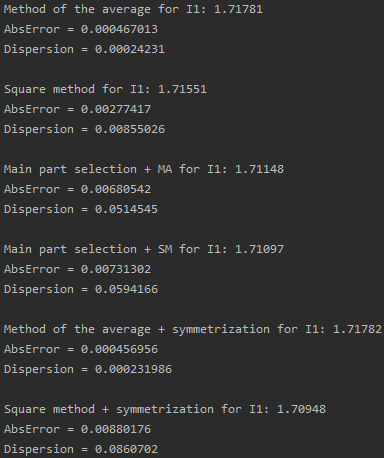
\includegraphics[width=0.85\linewidth]{I1}} a) \\
\end{minipage}
\hfill
\begin{minipage}[h]{0.47\linewidth}
\center{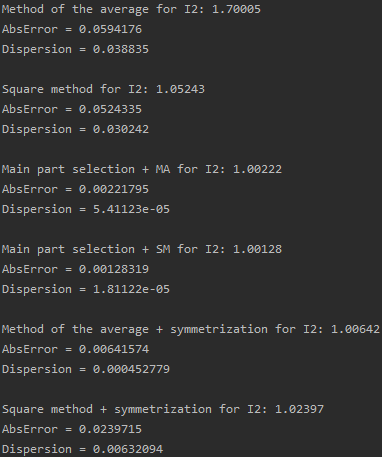
\includegraphics[width=0.85\linewidth]{I2}} b) \\
\end{minipage}
\vfill
\begin{minipage}[h]{1\linewidth}
\center{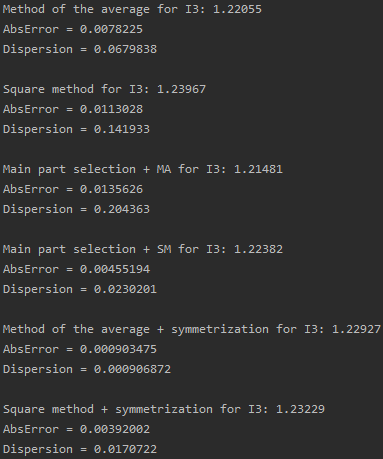
\includegraphics[width=0.44\linewidth]{I3}} c) \\
\end{minipage}
\vfill
\caption{Полученные значения интегралов, абсолютные величины ошибок вычисления и оценки дисперсии при расчёте методами среднего значения и площадей, используя следующие способы понижения дисперсии: выделение главной части и симметризация подынтегральной функции для $N = 10000$\\
a) $\int_{0}^{1}\exp(x)dx$, b) $\int_{0}^{\frac{\pi}{2}} \sin(x)dx$, c) $\int_{0}^{\sqrt{3}} x\arctan(x)dx$.}
\label{ris:1}
\end{figure}

\newpage
\subsection{Сравнение ММК с формулами среднего, трапеций, Симпсона и экстраполяцией Ричардсона для формулы Симпсона}
\begin{figure}[h]
\begin{minipage}[h]{0.48\linewidth}
\center{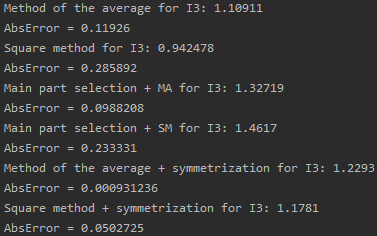
\includegraphics[width=1\linewidth]{I3_100}} a) \\
\end{minipage}
\hfill
\begin{minipage}[h]{0.48\linewidth}
\center{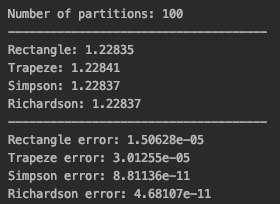
\includegraphics[width=1\linewidth]{N100}} b) \\
\end{minipage}
\hfill
\caption{Результаты вычисления интеграла $\int_{0}^{\sqrt{3}} x\arctan(x)dx$ a) ММК, б) формулами среднего, трапеций, Симпсона и экстраполяцией Ричардсона формулы Симпсона для $N = 100$.}
\label{ris:2}
\end{figure}

\newpage
\section{Вывод}
Был произведен расчёт интегралов $\int_{0}^{1}\exp(x)dx$, $\int_{0}^{\frac{\pi}{2}} \sin(x)dx$, $\int_{0}^{\sqrt{3}} x\arctan(x)dx$ методом Монте-Карло, используя методы вычисления среднего значения и площади, а также способы понижения дисперсии: выделение главной части и симметризация.

Благодаря способам понижения дисперсии в некоторых случаях удалось сократить величину ошибки на несколько порядков.

Из сравнения результатов, полученных использованием формул среднего, трапеций, Симпсона и экстраполяции Ричардсона для формулы Симпсона, и результатов, полученных применением ММК, очевидно, что точность расчета одномерных интегралов ММК существенно меньше: минимальная полученная величина ошибки ММК при вычислении интеграла $\int_{0}^{\sqrt{3}} x\arctan(x)dx$ имеет величину $9.31236\cdot 10^{-4}$, когда максимальная полученная величина ошибки для наименее точной из квадратурных формул, формулы прямоугольников, имеет величину $1.50628\cdot 10^{-5}$ при $N=100$.




\end{document} 